\section{Magic State Distillation}
\label{sec:magic}

Now we come to a beautiful idea which combines a geometric picture of
quantum computing with error correction, circuit construction, the idea of
using uninitialized quantum states, and architecture.
This idea is the \emph{magic state}.

In 2004, Bravyi and Kitaev proposed an interesting model of computation where
we assume we are able to perform the following set of operations $O$
perfectly: all the Clifford group operations,
prepare fiducial state $\ket{0}$, perform Pauli measurements, but in
addition we are given multiple copies of some mixed state $\rho$
\cite{Bravyi2004}. This last
is a parameter of our model. Under what conditions of $\rho$ are we still
able to do universal quantum computation (\textsc{UQC})? It turns out that
if $\rho$ is a pure state corresponding to the eigenstates of the Hadamard
($H$) operator or the $T$ operator, as defined below, then combined with the
above operations we are able to perform \textsc{UQC}. Note that the
$T$ operator here is \emph{not} the same as $R_Z{\pi/8}$ defined in
\ref{subsec:universal} that is
often called $T$ in the literature, for example in \cite{Nielsen2000}.

\begin{equation}
T = e^{i\pi / 4} KH = \frac{e^{i\pi/4}}{\sqrt{2}}
\left[ \begin{array}{cc}
1 & 1\\
i & -i
\end{array} \right]
\end{equation}

We denote by $\ket{H}$ and $\ket{T}$ the $+1$ eigenstates of $H$ and $T$
respectively. By the Clifford group operations, there are eight symmetric
magic states to $\ket{H}$ and twelve symmetric magic states to $\ket{T}$,
or $20$ magic states total. We will therefore distinguish between
magic states in the $\ket{H}$ direction, which can be identified as vectors
which go from the origin of the Bloch sphere to bisect the edges of the
Clifford octahedron, and magic states in the $\ket{T}$ direction, which
go through the centers of the faces of the Clifford octahedron.

\begin{equation}
\ket{T} = \cos(\theta) \ket{0} + e^{i\pi / 4}\sin(\theta) \ket{1} \qquad
\cos(2\theta) = \frac{1}{\sqrt{3}}
\end{equation}

\begin{equation}
\ket{H} = \ket{0} + e^{i\pi/4} \ket{1}
\end{equation}

The use of the word ``magic state'' in the error-correcting literature,
particularly for topological quantum computing, often refers to $\ket{H}$,
because it is useful for enacting the $R_Z(\pi/8)$ gate fault-tolerantly,
for most error-correcting codes which are able to do
the Clifford gates fault-tolerantly (and transversally).
%A circuit for doing this in the Steane code is shown in Figure \ref{fig:steane-pi8}.

%%%%%%%%%%
% FIGURE %
%%%%%%%%%%
%\begin{figure}
%\label{fig:steane-pi8}
%\caption{Fault-tolerant implementation of the $\pi/8$ gate using an $\ket{H}$-type
%magic state in the Steane code. \cite{Fowler2003}.}
%\end{figure}

%%%%%%%%%%%%%%%%%%%%%%%%%%%%%%%%%%%%%%%%%%%%%%%%%%%%%%%%%%%%%%%%%%%%%%%%%%%%%%
\subsection{Bloch Sphere}

We now return to the picture of the Bloch sphere from a previous section.
Whereas before we only considered pure states, those whose preparation could
be described in a deterministic way, this is not the most general definition
of a quantum state. In general, we may not know how a state was prepared,
either because a random error has occurred, or an adversary has tampered
maliciously with it, or because the original experimentalist who prepared
for the state for us is now unfortunately dead. This more general state,
called a \emph{mixed state}, can be expressed as a probabilistic ensemble of
states $\rho$, which is now a $2^n \times 2^n$ density matrix. All the
rules of quantum mechanics from the introduction can be reformulated in
terms of density matrices. For this report,
we will limit ourselves to single-qubit states with the understanding that
the framework generalizes naturally to multi-qubit states.

Although we
will not delve deeply into the properties of density matrices here, they are
a tool especially well-suited to expressing quantum states which are part
of a larger system which may be unknown. Here is where philosophers or
physicists who work in the foundations of quantum mechanics argue about whether
quantum states represent objective states of nature or simply our beliefs about
these states and the imperfect information we have about them. We will leave
that debate to them.

\begin{displaymath}
\rho = \sum_{j} p_j \ket{\psi_j}\bra{\psi_j}
\end{displaymath}

Here the probabilities $p_j$ should sum to $1$ to be a true probability
distribution. This is also how a mixed quantum state can be viewed as a
generalization of a classical probability distribution. In fact, many
quantum algorithms involve the ability to sample from a ``hard'' distribution,
that is, one that cannot even be sampled from efficiently using a classical
probabilistic algorithm, let alone generate the complete distribution itself.
%(Citation needed here, and also fact-checking. For example, sampling from
%the Gibbs distribution may not involved mixed states at all, like the
%quantum-quantum Metropolis algorithm).

In general, a mixed state can be expressed as a combination of the Pauli
matrices.

\begin{equation}
\rho = \frac{1}{2}(I + p_x\sigma_x + p_y\sigma_y + p_z\sigma_z)
\end{equation}

The values $(p_x, p_y, p_z)$ is known as the \emph{polarization vector} of
the mixed state and corresponds to its geometric three-dimensional coordinates
within the Bloch sphere (now properly considered a Bloch ball, since mixed
states can occupy the interior of the ball's volume). The real numbers
$p_x$, $p_y$, and $p_z$ lie in the range $[-1,1]$.

Mixed states include the pure states as a special case, that is, all the
points that lie on the Bloch sphere surface. To restrict mixed states
to those points which lie within the Bloch ball, including the surface,
we impose $|p_x| + |p_y| + |p_z| \le 1$.

%We can also describe the
%correspondence between the polarization vector and our conventional
%description of a quantum state as follows.

%\begin{equation}
%\end{equation}

It turns out, by using the stabilizer framework (note here that stabilizer
framework should come before this section) and the Gottesman-Knill theorem,
we can classically simulate all the states within the interior of an
\emph{octahedron}, which we will call $\mathcal{O}$, which is defined as the
convex hull of the six points corresponding to the eigenstates of the
$X$, $Y$, and $Z$ operators.
This is shown in Figure \ref{fig:clifford-octahedron}.
These therefore known as stabilizer states, and we will sometimes refer to
$\mathcal{O}$ as the Clifford octahedron because all of these states can be
reached using the operations in $O$, which include the $\mathcal{C}_1$.
Note to self, this section should come after the section explaining the
Clifford group. It is therefore not surprising, although still somewhat
mysterious, that the 24 elements of the $\mathcal{C}_1$ correspond
exactly to the symmetries of the octahedron. (I think this is $S_4$, this
could use some fact-checking love).

\begin{figure}
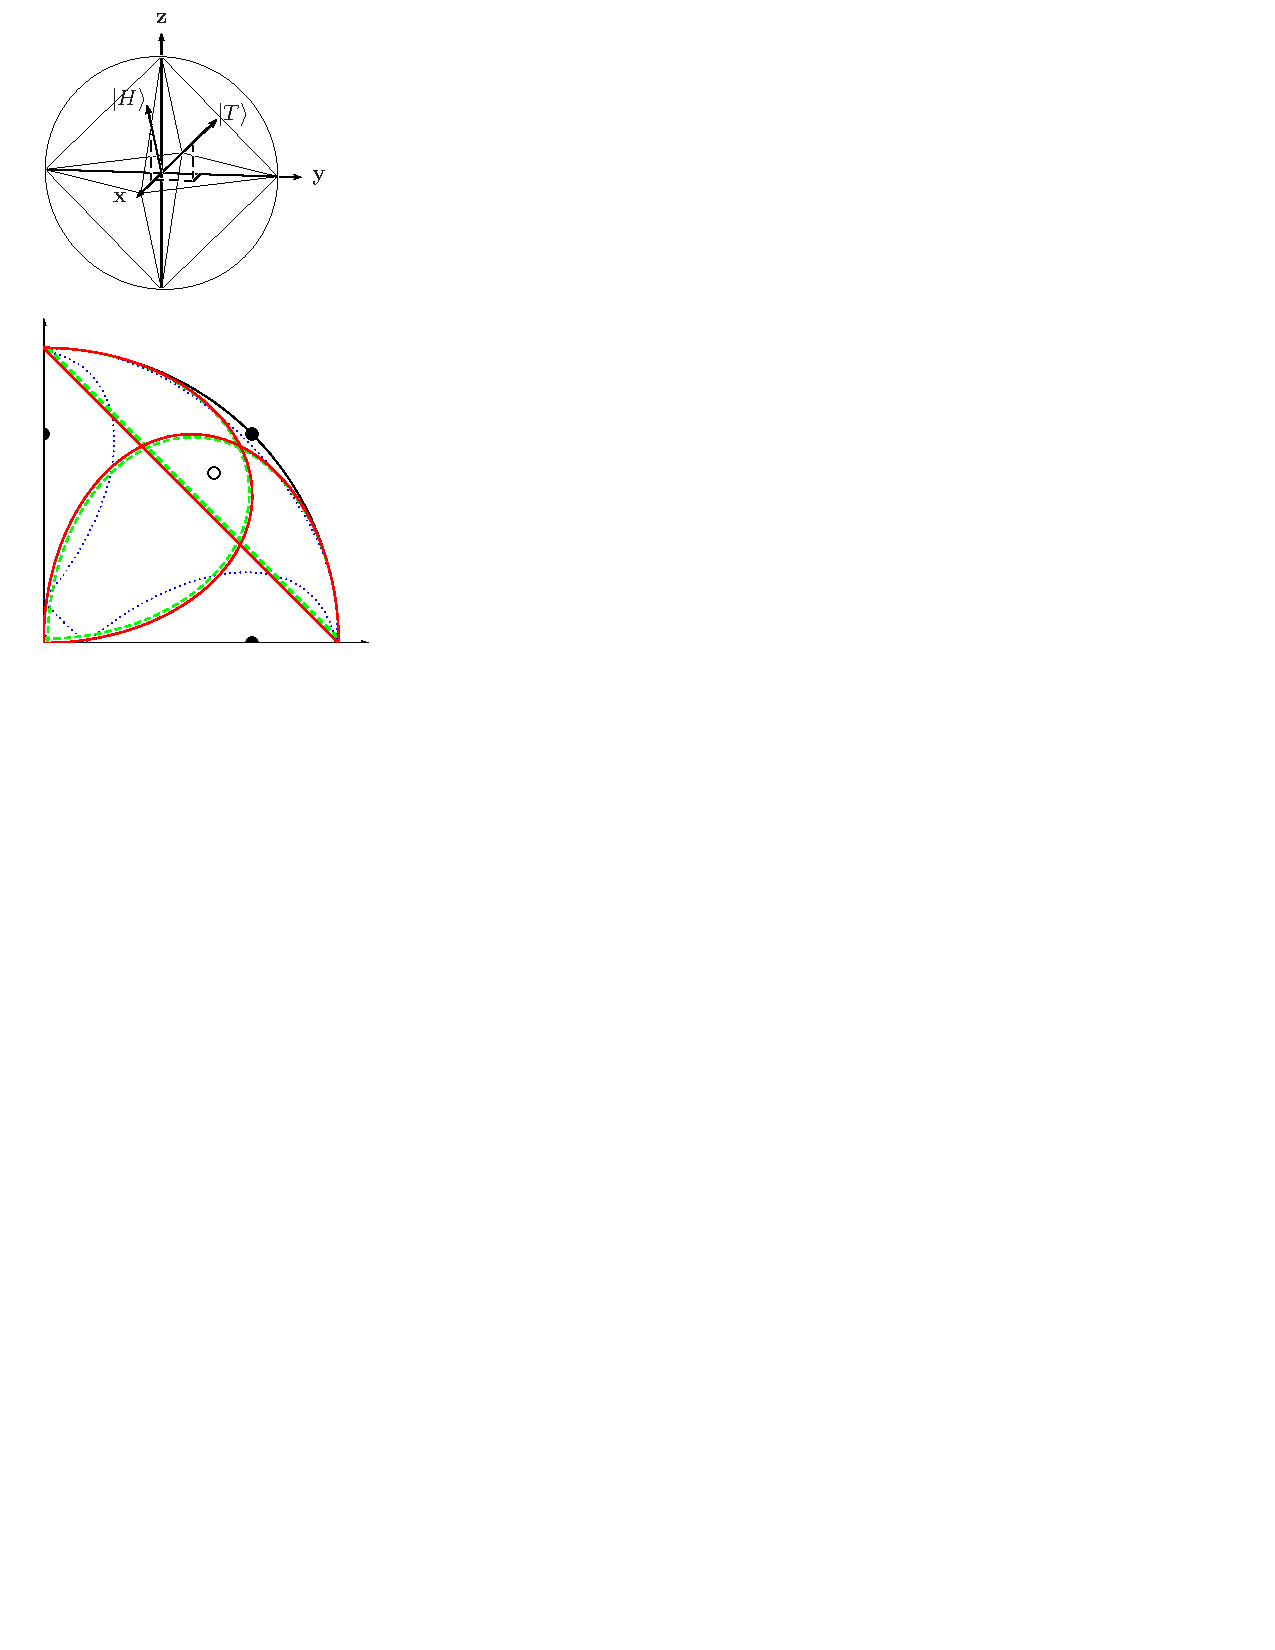
\includegraphics[width=3in]{figures/blochsphere.pdf}
\caption{The Bloch sphere with octahedron $\mathcal{O}$ and the magic states
$\ket{T}$ and $\ket{H}$.}
\label{fig:clifford-octahedron}
\end{figure}

%%%%%%%%%%%%%%%%%%%%%%%%%%%%%%%%%%%%%%%%%%%%%%%%%%%%%%%%%%%%%%%%%%%%%%%%%%%%%%
\subsection{Error Decoding}

The process of magic state distillation is actually just
concatenated error decoding, where the decoder we use determines how many
copies of the state $\rho$ we need and what polarization threshold we can
tolerate and still get a magic state. For example, in Bravyi and 
Kitaev's original paper \cite{Bravyi2004} they used the well-known 5-qubit
code to distill from five copies of $\rho$ in the $\ket{T}$ direction.
The resulting threshold condition is that all $\rho$ that lies beyond the plane
parallel to a face of $\mathcal{O}$ at distance $\approx 0.665$ from the
origin can efficiently be corrected to $\ket{T}$, by recursively applying
concatenated layers of the 5-qubit decoder.

In that scenario, we prepare our $\rho$ ``noisily'' by
randomly applying the unitary $T$ with probability $p$.
Then each $\rho$ is a mixture of the $e^{2\pi i / 3}$ and
$e^{-2\pi i / 3}$ eigenstates of $T$ with probabilities $(1-p)$ and $p$.
Just like with the fault-tolerant
threshold theorem, every application of magic state distillation for a
sufficiently small $p$ will result in an output state $\rho$ that is closer
to $\ket{T}$, that is, $p_{out} < p$, according to Equation
\ref{eqn:p_out}.

\begin{equation}
p_{out} = \frac{t^5 + 5t^2}{1 + 5t^2 + 5t^3 + t^5} \qquad t \equiv \frac{p}{1-p}
\label{eqn:p_out}
\end{equation}

This threshold then divides up the Bloch ball into regions which can eventually
be distilled to a magic state, either in the $\ket{H}$-direction or the
$\ket{T}$-direction, and those which cannot. A threshold is \emph{tight}
if it exactly defines a surface inside which $\rho$ cannot be distilled to
a magic state and is also classically-simulatable. Definitely
we know that states within the Clifford octahedron $\mathcal{O}$ belong to this
latter category, and that the points on the sphere corresponding to
$\ket{H}$ and $\ket{T}$ have unquestionable magicness.

We know that there is a tight separation in the $\ket{H}$ direction 
corresponding to $p \approx 14.64\%$ due to Reichardt \cite{Reichardt2004}.
However, there is not a tight-separation in the $\ket{T}$ direction. There
is an ambiguous region between the planes that lie $0.655$ and $0.577$
from the origin, parallel to the face of $\mathcal{O}$, where it is neither
known whether distillation is possible nor whether these states can be used
to perform \textsf{UQC}. This is an interesting open question.

%\subsection{Practical Application / Uninitialized Qubits}

%That's great, you may be thinking, but magic is fake. It certainly isn't a good
%name if I want to build actual working quantum computers. Well, it turns out
%that magic state distillation is an important part of several physical approaches
%to building a quantum computer. This importance comes from the fact that the
%$\pi/8$ gate is not efficient to implement in a fault-tolerant way directly
%in either topological codes (including the Kitaev surface code), many CSS
%codes used for concatenated error correction, and even in physically
%topological systems such as those using the fractional quantum Hall effect.
%(cite Station Q papers here).

%What we can do is, using a (possibly large) number of uninitialized qubits
%in some mixed state, distill them into a magic state $\ket{H}$ as an ancillary
%resource to our normal circuit. Whenever we need to apply a $\pi/8$ gate to
%a qubit, we make it the target of a CNOT controlled on our distilled magic
%state $\ket{H}$. Therefore, there is a big area of quantum architecture which
%becomes then, how to design around this large areas where magic state
%distillation needs to happen, and where magic states need to be inserted
%into the system. This depends on practical error rates and the number of
%distillation layers needed, as determined below.

%There is also a lot of work experimentally to be done. It could be that the
%thresholds above in the previous section are nonsense, because empirically,
%it is possible or easy to distill magic states. This can only be done
%by trial and error (fact-check? maybe think about this statement some more?)

